\documentclass[UTF8,12pt]{article}
\usepackage[utf8]{inputenc}
\usepackage[T1]{fontenc}
\usepackage{vmargin} % page format
\usepackage{soul}       % underline multiple lines
\usepackage{enumerate}
\usepackage{enumitem}
\usepackage{color}
\usepackage{amsmath}
\usepackage{multirow}
\usepackage{amssymb}
\usepackage{bbm}
\usepackage{graphicx}
\usepackage{subfig}
\usepackage{diagbox}
\usepackage[pdfstartview=FitH,
CJKbookmarks=true,
bookmarksnumbered=true,
bookmarksopen=true,
colorlinks=true,                        
linkcolor=black]{hyperref}
\usepackage[numbers]{natbib}
\newcommand{\sinc}{\mathrm{sinc}}
\setpapersize{USletter}
\setmarginsrb{1 in}{1 in}{1 in}{0.5 in}{0pt}{0mm}{0pt}{0.5 in}
\pagestyle{empty}
\pagestyle{plain}
\setlength{\parskip}{1em}
\renewcommand{\baselinestretch}{1.5}
\usepackage{sectsty}% section font size
\usepackage{titlesec}% section spacing
\sectionfont{\fontsize{12}{0}\selectfont}
\subsectionfont{\fontsize{12}{0}\selectfont}
\titlespacing\section{0pt}{12pt plus 4pt minus 2pt}{0pt plus 2pt minus 2pt}
\titlespacing\subsection{0pt}{12pt plus 4pt minus 2pt}{0pt plus 2pt minus 2pt}
\titlespacing\subsubsection{0pt}{12pt plus 4pt minus 2pt}{0pt plus 2pt minus 2pt}

\title{Predicting Hand-written Digits using Support Vector Machines (SVM)}
\date{2019\\ March}
\author{Yue WU\\ yw9998\\CS 391L}
\begin{document}
	\maketitle
	\section{Introduction}
	This homework aims at using Support Vector Machines (SVM) to detect hand-written digits automatically. We will use a certain amount (ntrain) of training images included in a training set of 60000 images to derive an algorithm that can detect the digits shown in a test set of 10000 images. Each image contains 784 pixels.
	\section{Methods}
	As Andrew Ng said in his lecture, "SVMs are among the best 'off-the-shelf' supervised learning algorithms." The algorithm not only tries to divide data into two groups using a linear classifier (or a hyperplane classifier for higher dimensions) as shown in Equation \ref{eq:linear classifier}, it also aims at maximizing the margin between the two groups (Equation \ref{eq:margin}). 
	\begin{equation}
	\label{eq:linear classifier}
	f(x) = \omega^{T}x+b
	\end{equation}
	\begin{equation}
	\label{eq:margin}
	\frac{\omega }{\left \| \omega  \right \|}\cdot \left ( x_{+}-x_{-} \right )=\frac{2}{\left \| \omega \right \|}
	\end{equation}
	Therefore, we arrive at the following optimization problem:
	\begin{equation}
	\begin{split}
	\min_{\omega,b}\ \ \frac{1}{2}\left \| \omega  \right \|^{2}\\
	y^{(i)}(\omega ^{T}x^{(i)}+b)\geq 1,\ i=1,...,m\\
	g_{i}(\omega )=-y^{(i)}(\omega ^{T}x^{(i)}+b)+1\leq 0
	\end{split}
	\end{equation}
	We also tried to reduce sensitivity to outliers by modifying the optimization problem as:
	\begin{equation}
	\begin{split}
	\min_{\gamma,\omega,b}\ \ \frac{1}{2}\left \| \omega  \right \|^{2}+C\sum_{i=1}^{m}\xi _{i}\\y^{(i)}(\omega ^{T}x^{(i)}+b)\geq 1-\xi _{i},\ i=1,...,m\\\xi_{i}\geq 0, \ i=1,...,m
	\end{split}
	\end{equation}
	When C is smaller, we call it a softer margin. When C is larger (C = 10000), we have a harder margin.
	The dual optimization problem is:
	\begin{equation}
	\label{eq:dual}
	\begin{split}
	\max_{\alpha}\ \ W(\alpha )=\sum_{i=1}^{m}\alpha _{i}-\frac{1}{2}\sum_{i,j=1}^{m}y^{(i)}y^{(j)}\alpha _{i}\alpha _{j}\left \langle x^{(i)}x^{(j)} \right \rangle\\0\leq \alpha _{i}\leq C,\ i=1,...,m\\sum_{i=1}^{m}\alpha _{i}y^{(i)}=0
	\end{split}
	\end{equation}
	For each image, values for the pixels are stored in a matrix named X (ntrain - 784), and the numbers of the group that each image belongs to are stored in a matrix named Y. The numbers stored in Y are called "labels." We will first train the algorithm by using the training set to calculate $\omega$ and b; then we can use Equation \ref{eq:predict} to predict the labels for the test set, and compare our prediction Z with actual labels Y to calculate the accuracy of the algorithm. Note that there is a kernel in the equation. In our study, we tried two kinds of kernels: polynomial kernels (Equation \ref{eq:poly}) and Gaussian kernels (Equation \ref{eq:rad}), and compared the difference in accuracy. 
	\begin{equation}
	\label{eq:predict}
	z=\omega ^{T}x+b
	\end{equation}
	\begin{equation}
	\label{eq:poly}
	K(x,z)=(\frac{1}{l^{2}}x^{T}z+1)^{p}
	\end{equation}
	\begin{equation}
	\label{eq:rad}
	K(x,z)=exp\left ( -\frac{\left \| x-z \right \|^{2}}{2\sigma ^{2}} \right )
	\end{equation}
	We also applied the Sequential Minimal Optimization (SMO) algorithm during the training. The SMO algorithm gives an efficient way of solving the dual problem of the SVM optimization problem (Equation \ref{eq:dual}). By applying the SMO algorithm, we 1) select two $\alpha$ parameters randomly, 2) find $\alpha _{j}$ so as to maximize the objective function, 3) solve for $\alpha _{i}$ using the value of $\alpha _{j}$, 4) calculate the b threshold.
	\section{Results}
	We first used the data set (4 vs 9), which is supposed to be one of the harder ones to classify, to determine the optimal values for sizes of both kernels. The code used is stored in \texttt{hw3\_compareplsig.m}. The number of training set is set to be 5000. Results are shown in Figure \ref{fig:pl} and figure \ref{fig:sig}. For polynomial kernels (Equation \ref{eq:poly}), as p increases, the values rapidly increases, therefore we need larger l to scale down the value in order to get reasonable results. In other words, l should increase with p. The optimal combination we chose here is p = 11 and l = 10. For Gaussian kernels (Equation \ref{eq:rad}), accuracy increases with $\sigma$ until $\sigma$ reaches 10, then accuracy starts to decrease. Therefore, we chose $\sigma$ = 10 as the optimal value.
	\begin{figure}[!ht]
		\centering
		\subfloat[]{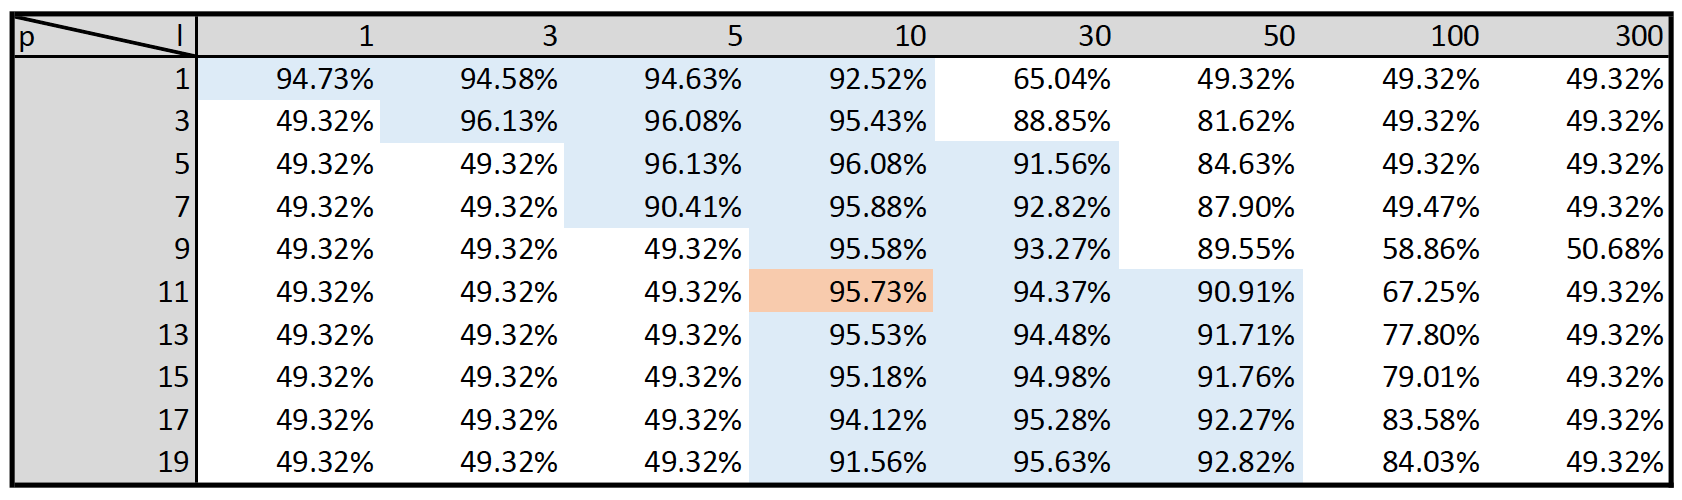
\includegraphics[width=1\linewidth]{figures/pl.png}}
		\caption{\label{fig:pl}Accuracies for different sizes of polynomial kernels. l increases from left to right, p increases from top to bottom. White color indicates low accuracy, blue color indicates high accuracy and orange indicate the combination we chose when applying the algorithm.}
	\end{figure}
	\begin{figure}[!ht]
		\centering
		\subfloat[]{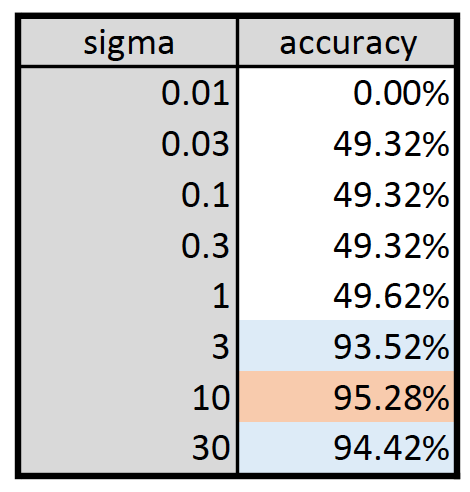
\includegraphics[width=0.25\linewidth]{figures/sig.png}}
		\caption{\label{fig:sig}Accuracies for different sizes of Gaussian kernels. $\sigma$ increases from top to bottom. White color indicates low accuracy, blue color indicates high accuracy and orange indicate the value of $\sigma$ we chose when applying the algorithm.}
	\end{figure}
	
	Next, we defined y = 1 and y = -1 for each case for both training set and test set and chose Cp and Cr for each case. The code used is stored in \texttt{hw3\_compareC.m}. The number of training set is set to be 2000. We manually input possible numbers for Cp and Cr (candidates) and the values for p, l, and $\sigma$ that we just found out, trained the algorithm, predicted the labels and calculated error percentage for all combinations of Cp and Cr. The one with the highest accuracy is chosen to be the optimal combination for one data set. The candidates and optimal Cps and Crs are shown in Figure \ref{fig:C}. We found out that for polynomial kernels, changes in C would not affect the accuracy much as the differences in error percentage between the softest margin and hardest margin are less than $1\%$. However, for Gaussian kernels, harder margin usually performs better. Differences in error percentage between the softest margin and hardest margin for easier cases ($\#1$ and $\#2$) are smaller, usually less than $6\%$. Differences in error percentage between the softest margin and hardest margin for harder cases ($\#3$, $\#4$ and $\#5$) are larger, which can range from $~50\%$ for softest margin to $1\%$ for hardest margin.
	\begin{figure}[!ht]
		\centering
		\subfloat[]{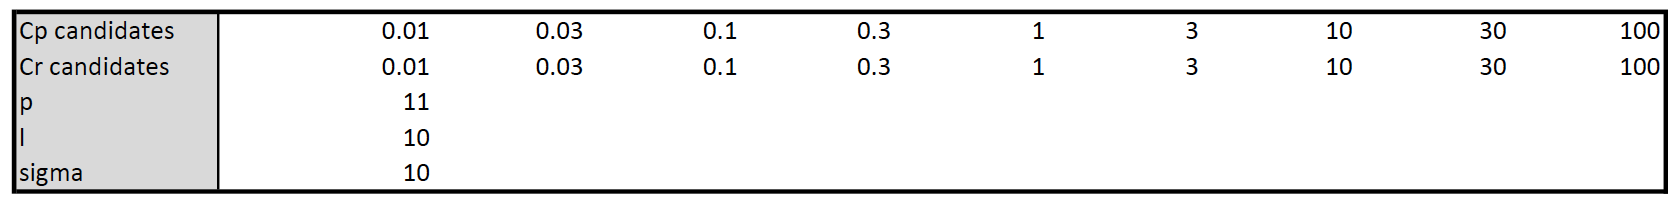
\includegraphics[width=1\linewidth]{figures/Ccandi.png}}\\
		\subfloat[]{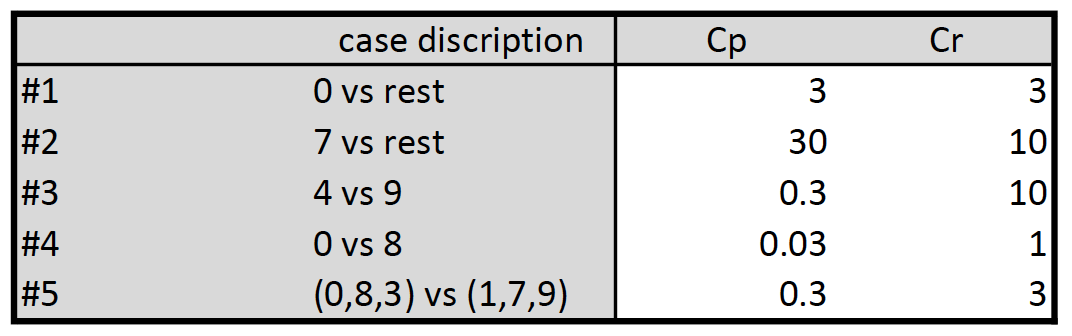
\includegraphics[width=0.5\linewidth]{figures/Coptimal.png}}
		\caption{\label{fig:C}(a) Candidates for Cp and Cr which the optimal values were chosen from, and the values of p, l, and $\sigma$ we used during the tests. (b) The optimal Cps and Crs for all five cases chosen by the tests.}
	\end{figure}
	
	We then compared between optimal margins, hard margins, and soft margins. The code used is stored in \texttt{hw3\_hardsoft.m}. We set the softer margin as $Cs = 0.01$, and the harder margin as $Ch = 1e5$. The number of the training set is set to be 5000. Values for p, l, and $\sigma$ are the ones we calculated before. Figure \ref{fig:hardsoft} shows the differences in accuracy using different margins, different kernels and among five cases. We noticed that 1) for polynomial kernels, changes in C won't affect the accuracy much although the harder margins were slightly better, while for Gaussian kernels, harder margins performed better as we have seen before, 2) the easier cases ($\#1$ and $\#2$) generally shown higher accuracy than the harder cases ($\#3$, $\#4$ and $\#5$), 3) accuracy differences between harder margins and softer margins were smaller for the easier cases ($\#1$ and $\#2$) compared to the harder cases ($\#3$, $\#4$ and $\#5$).
	\begin{figure}[!ht]
		\centering
		\subfloat[]{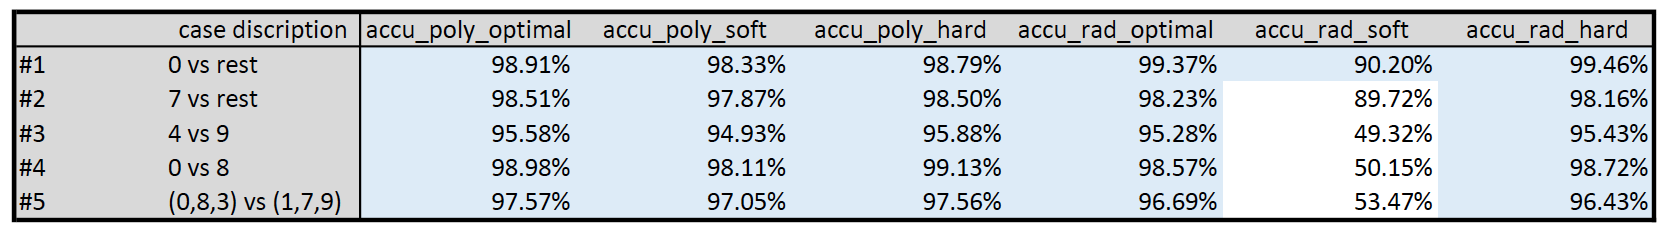
\includegraphics[width=1\linewidth]{figures/hardsoft.png}}
		\caption{\label{fig:hardsoft}Accuracies for different sizes of Gaussian kernels. $\sigma$ increases from top to bottom. White color indicates low accuracy, blue color indicates high accuracy and orange indicate the value of $\sigma$ we chose when applying the algorithm.}
	\end{figure}
	\section{Conclusion and discussion}
	The values for p, l, and $\sigma$ can largely affect accuracy. For polynomial kernels, after finding a suitable p for a data set, the value of l should correlate well with p so that the values are best scaled. For Gaussian kernels, accuracy usually increases with $\sigma$ to a maximum number, and then drops.
	
	For our study, harder margins usually perform better. The reason might be that the data is easy to be distinguished from the others (the margins are already clear), in which case increasing tolerance for outliers will only cause more misclassification. Whether the margin is hard or soft affects Gaussian kernels much more than polynomial kernels, and differences in accuracy caused by different margins are larger for harder cases.
	
	Easier cases generally show larger accuracy for harder cases, but this does not guarantee that our algorithm always performs better for easier cases because we also need to take account the total number of appearance of the target group in the whole data set. As we can see in Figure \ref{fig:hardsoft}, when we used a softer margin for Gaussian kernel, the easier cases  ($\#1$ and $\#2$) still shown accuracies as high as $~90\%$, while accuracies for harder cases ($\#3$, $\#4$ and $\#5$) were only $~50\%$. It looks like the algorithm still succeeded in the easier cases, but it was not. For the easier cases, our target groups were 0 and 7, and both took up only $10\%$ in the whole dataset. Even the algorithm did not predict any target number correctly we could still achieve an accuracy of $~90\%$. Therefore, an accuracy of $~90\%$ for the easier cases and an accuracy of $~50\%$ for the harder cases both indicate failures in prediction.
	
\end{document}